% Created by tikzDevice version 0.9 on 2016-01-13 23:40:08
% !TEX encoding = UTF-8 Unicode
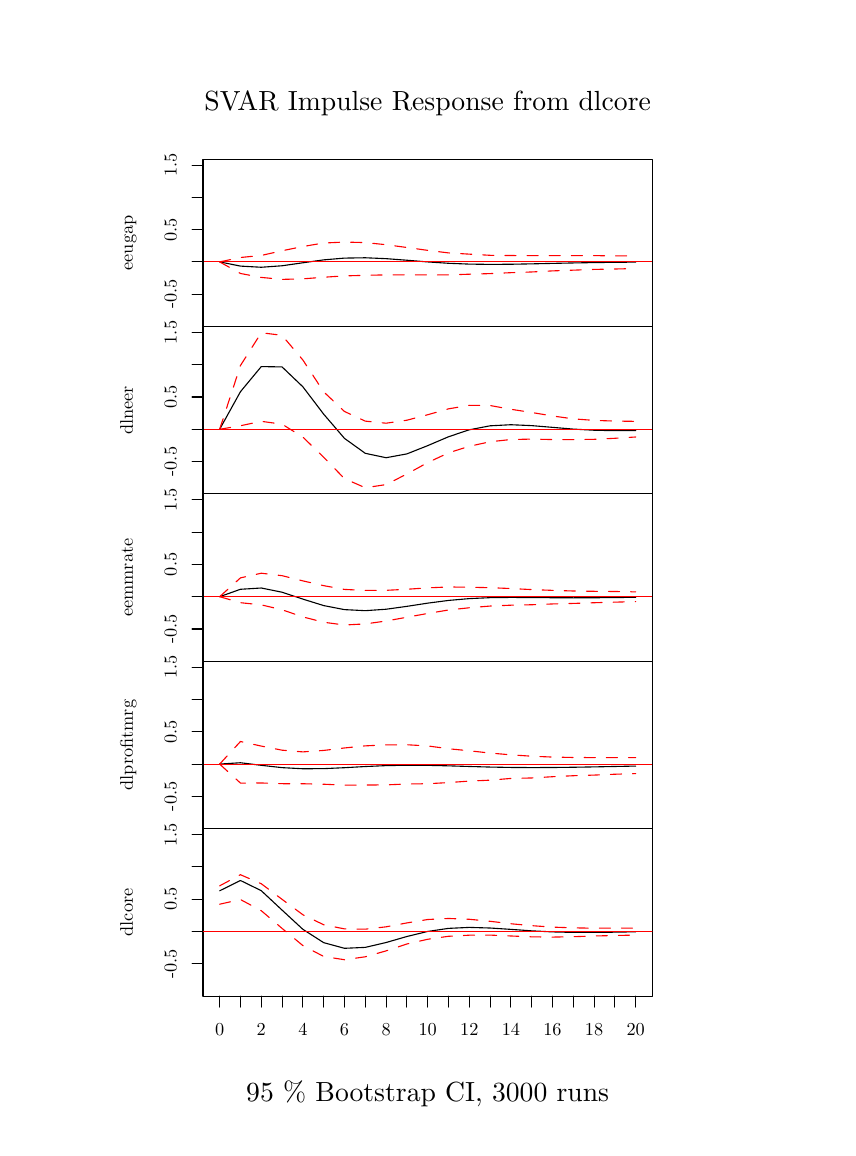
\begin{tikzpicture}[x=1pt,y=1pt]
\definecolor{fillColor}{RGB}{255,255,255}
\path[use as bounding box,fill=fillColor,fill opacity=0.00] (0,0) rectangle (289.08,397.48);
\begin{scope}
\path[clip] ( 63.36,289.48) rectangle (225.72,349.96);
\definecolor{drawColor}{RGB}{0,0,0}

\path[draw=drawColor,line width= 0.4pt,line join=round,line cap=round] ( 69.37,312.84) --
	( 76.89,311.32) --
	( 84.41,310.90) --
	( 91.92,311.44) --
	( 99.44,312.52) --
	(106.96,313.57) --
	(114.47,314.21) --
	(121.99,314.33) --
	(129.51,314.01) --
	(137.02,313.44) --
	(144.54,312.83) --
	(152.06,312.34) --
	(159.57,312.04) --
	(167.09,311.94) --
	(174.61,311.99) --
	(182.12,312.13) --
	(189.64,312.30) --
	(197.16,312.46) --
	(204.67,312.59) --
	(212.19,312.69) --
	(219.71,312.76);
\end{scope}
\begin{scope}
\path[clip] ( 31.68,289.48) rectangle (257.40,349.96);
\definecolor{drawColor}{RGB}{0,0,0}

\node[text=drawColor,anchor=base,inner sep=0pt, outer sep=0pt, scale=  0.66] at (144.54,259.38) {xy{\$}x};

\node[text=drawColor,rotate= 90.00,anchor=base,inner sep=0pt, outer sep=0pt, scale=  0.66] at ( 38.02,319.72) {eeugap};
\end{scope}
\begin{scope}
\path[clip] (  0.00,  0.00) rectangle (289.08,397.48);
\definecolor{drawColor}{RGB}{0,0,0}

\path[draw=drawColor,line width= 0.4pt,line join=round,line cap=round] ( 63.36,301.18) -- ( 63.36,347.82);

\path[draw=drawColor,line width= 0.4pt,line join=round,line cap=round] ( 63.36,301.18) -- ( 59.40,301.18);

\path[draw=drawColor,line width= 0.4pt,line join=round,line cap=round] ( 63.36,312.84) -- ( 59.40,312.84);

\path[draw=drawColor,line width= 0.4pt,line join=round,line cap=round] ( 63.36,324.50) -- ( 59.40,324.50);

\path[draw=drawColor,line width= 0.4pt,line join=round,line cap=round] ( 63.36,336.16) -- ( 59.40,336.16);

\path[draw=drawColor,line width= 0.4pt,line join=round,line cap=round] ( 63.36,347.82) -- ( 59.40,347.82);

\node[text=drawColor,rotate= 90.00,anchor=base,inner sep=0pt, outer sep=0pt, scale=  0.66] at ( 53.86,301.18) {-0.5};

\node[text=drawColor,rotate= 90.00,anchor=base,inner sep=0pt, outer sep=0pt, scale=  0.66] at ( 53.86,324.50) {0.5};

\node[text=drawColor,rotate= 90.00,anchor=base,inner sep=0pt, outer sep=0pt, scale=  0.66] at ( 53.86,347.82) {1.5};
\end{scope}
\begin{scope}
\path[clip] ( 63.36,289.48) rectangle (225.72,349.96);
\definecolor{drawColor}{RGB}{255,0,0}

\path[draw=drawColor,line width= 0.4pt,line join=round,line cap=round] ( 63.36,312.84) -- (225.72,312.84);

\path[draw=drawColor,line width= 0.4pt,dash pattern=on 4pt off 4pt ,line join=round,line cap=round] ( 69.37,312.84) --
	( 76.89,314.43) --
	( 84.41,315.17) --
	( 91.92,316.86) --
	( 99.44,318.40) --
	(106.96,319.66) --
	(114.47,320.00) --
	(121.99,319.82) --
	(129.51,319.05) --
	(137.02,318.05) --
	(144.54,317.01) --
	(152.06,316.09) --
	(159.57,315.64) --
	(167.09,315.22) --
	(174.61,315.14) --
	(182.12,315.09) --
	(189.64,315.10) --
	(197.16,315.13) --
	(204.67,315.11) --
	(212.19,315.01) --
	(219.71,314.98);

\path[draw=drawColor,line width= 0.4pt,dash pattern=on 4pt off 4pt ,line join=round,line cap=round] ( 69.37,312.84) --
	( 76.89,308.65) --
	( 84.41,307.23) --
	( 91.92,306.52) --
	( 99.44,306.71) --
	(106.96,307.30) --
	(114.47,307.78) --
	(121.99,307.99) --
	(129.51,308.15) --
	(137.02,308.14) --
	(144.54,308.14) --
	(152.06,308.14) --
	(159.57,308.39) --
	(167.09,308.61) --
	(174.61,308.94) --
	(182.12,309.20) --
	(189.64,309.59) --
	(197.16,309.85) --
	(204.67,310.12) --
	(212.19,310.27) --
	(219.71,310.44);
\end{scope}
\begin{scope}
\path[clip] (  0.00,  0.00) rectangle (289.08,397.48);
\definecolor{drawColor}{RGB}{0,0,0}

\path[draw=drawColor,line width= 0.4pt,line join=round,line cap=round] ( 63.36,289.48) --
	(225.72,289.48) --
	(225.72,349.96) --
	( 63.36,349.96) --
	( 63.36,289.48);
\end{scope}
\begin{scope}
\path[clip] ( 63.36,228.99) rectangle (225.72,289.48);
\definecolor{drawColor}{RGB}{0,0,0}

\path[draw=drawColor,line width= 0.4pt,line join=round,line cap=round] ( 69.37,252.35) --
	( 76.89,265.94) --
	( 84.41,275.01) --
	( 91.92,274.89) --
	( 99.44,267.71) --
	(106.96,257.82) --
	(114.47,249.07) --
	(121.99,243.67) --
	(129.51,242.08) --
	(137.02,243.46) --
	(144.54,246.44) --
	(152.06,249.65) --
	(159.57,252.17) --
	(167.09,253.61) --
	(174.61,254.00) --
	(182.12,253.68) --
	(189.64,253.05) --
	(197.16,252.42) --
	(204.67,252.01) --
	(212.19,251.85) --
	(219.71,251.91);
\end{scope}
\begin{scope}
\path[clip] ( 31.68,228.99) rectangle (257.40,289.48);
\definecolor{drawColor}{RGB}{0,0,0}

\node[text=drawColor,anchor=base,inner sep=0pt, outer sep=0pt, scale=  0.66] at (144.54,198.89) {xy{\$}x};

\node[text=drawColor,rotate= 90.00,anchor=base,inner sep=0pt, outer sep=0pt, scale=  0.66] at ( 38.02,259.23) {dlneer};
\end{scope}
\begin{scope}
\path[clip] (  0.00,  0.00) rectangle (289.08,397.48);
\definecolor{drawColor}{RGB}{0,0,0}

\path[draw=drawColor,line width= 0.4pt,line join=round,line cap=round] ( 63.36,240.69) -- ( 63.36,287.33);

\path[draw=drawColor,line width= 0.4pt,line join=round,line cap=round] ( 63.36,240.69) -- ( 59.40,240.69);

\path[draw=drawColor,line width= 0.4pt,line join=round,line cap=round] ( 63.36,252.35) -- ( 59.40,252.35);

\path[draw=drawColor,line width= 0.4pt,line join=round,line cap=round] ( 63.36,264.01) -- ( 59.40,264.01);

\path[draw=drawColor,line width= 0.4pt,line join=round,line cap=round] ( 63.36,275.67) -- ( 59.40,275.67);

\path[draw=drawColor,line width= 0.4pt,line join=round,line cap=round] ( 63.36,287.33) -- ( 59.40,287.33);

\node[text=drawColor,rotate= 90.00,anchor=base,inner sep=0pt, outer sep=0pt, scale=  0.66] at ( 53.86,240.69) {-0.5};

\node[text=drawColor,rotate= 90.00,anchor=base,inner sep=0pt, outer sep=0pt, scale=  0.66] at ( 53.86,264.01) {0.5};

\node[text=drawColor,rotate= 90.00,anchor=base,inner sep=0pt, outer sep=0pt, scale=  0.66] at ( 53.86,287.33) {1.5};
\end{scope}
\begin{scope}
\path[clip] ( 63.36,228.99) rectangle (225.72,289.48);
\definecolor{drawColor}{RGB}{255,0,0}

\path[draw=drawColor,line width= 0.4pt,line join=round,line cap=round] ( 63.36,252.35) -- (225.72,252.35);

\path[draw=drawColor,line width= 0.4pt,dash pattern=on 4pt off 4pt ,line join=round,line cap=round] ( 69.37,252.35) --
	( 76.89,275.40) --
	( 84.41,287.24) --
	( 91.92,286.30) --
	( 99.44,277.39) --
	(106.96,265.89) --
	(114.47,258.79) --
	(121.99,255.30) --
	(129.51,254.55) --
	(137.02,255.63) --
	(144.54,257.61) --
	(152.06,259.74) --
	(159.57,261.02) --
	(167.09,260.94) --
	(174.61,259.58) --
	(182.12,258.43) --
	(189.64,257.17) --
	(197.16,256.12) --
	(204.67,255.57) --
	(212.19,255.32) --
	(219.71,255.22);

\path[draw=drawColor,line width= 0.4pt,dash pattern=on 4pt off 4pt ,line join=round,line cap=round] ( 69.37,252.35) --
	( 76.89,253.63) --
	( 84.41,255.23) --
	( 91.92,254.20) --
	( 99.44,249.53) --
	(106.96,242.25) --
	(114.47,234.52) --
	(121.99,231.23) --
	(129.51,232.37) --
	(137.02,236.20) --
	(144.54,240.31) --
	(152.06,243.84) --
	(159.57,246.21) --
	(167.09,247.85) --
	(174.61,248.65) --
	(182.12,248.81) --
	(189.64,248.64) --
	(197.16,248.62) --
	(204.67,248.73) --
	(212.19,249.10) --
	(219.71,249.57);
\end{scope}
\begin{scope}
\path[clip] (  0.00,  0.00) rectangle (289.08,397.48);
\definecolor{drawColor}{RGB}{0,0,0}

\path[draw=drawColor,line width= 0.4pt,line join=round,line cap=round] ( 63.36,228.99) --
	(225.72,228.99) --
	(225.72,289.48) --
	( 63.36,289.48) --
	( 63.36,228.99);
\end{scope}
\begin{scope}
\path[clip] ( 63.36,168.50) rectangle (225.72,228.99);
\definecolor{drawColor}{RGB}{0,0,0}

\path[draw=drawColor,line width= 0.4pt,line join=round,line cap=round] ( 69.37,191.86) --
	( 76.89,194.54) --
	( 84.41,195.00) --
	( 91.92,193.48) --
	( 99.44,190.99) --
	(106.96,188.65) --
	(114.47,187.19) --
	(121.99,186.81) --
	(129.51,187.33) --
	(137.02,188.37) --
	(144.54,189.53) --
	(152.06,190.51) --
	(159.57,191.17) --
	(167.09,191.51) --
	(174.61,191.60) --
	(182.12,191.56) --
	(189.64,191.49) --
	(197.16,191.46) --
	(204.67,191.48) --
	(212.19,191.55) --
	(219.71,191.64);
\end{scope}
\begin{scope}
\path[clip] ( 31.68,168.50) rectangle (257.40,228.99);
\definecolor{drawColor}{RGB}{0,0,0}

\node[text=drawColor,anchor=base,inner sep=0pt, outer sep=0pt, scale=  0.66] at (144.54,138.40) {xy{\$}x};

\node[text=drawColor,rotate= 90.00,anchor=base,inner sep=0pt, outer sep=0pt, scale=  0.66] at ( 38.02,198.74) {eemmrate};
\end{scope}
\begin{scope}
\path[clip] (  0.00,  0.00) rectangle (289.08,397.48);
\definecolor{drawColor}{RGB}{0,0,0}

\path[draw=drawColor,line width= 0.4pt,line join=round,line cap=round] ( 63.36,180.20) -- ( 63.36,226.84);

\path[draw=drawColor,line width= 0.4pt,line join=round,line cap=round] ( 63.36,180.20) -- ( 59.40,180.20);

\path[draw=drawColor,line width= 0.4pt,line join=round,line cap=round] ( 63.36,191.86) -- ( 59.40,191.86);

\path[draw=drawColor,line width= 0.4pt,line join=round,line cap=round] ( 63.36,203.52) -- ( 59.40,203.52);

\path[draw=drawColor,line width= 0.4pt,line join=round,line cap=round] ( 63.36,215.18) -- ( 59.40,215.18);

\path[draw=drawColor,line width= 0.4pt,line join=round,line cap=round] ( 63.36,226.84) -- ( 59.40,226.84);

\node[text=drawColor,rotate= 90.00,anchor=base,inner sep=0pt, outer sep=0pt, scale=  0.66] at ( 53.86,180.20) {-0.5};

\node[text=drawColor,rotate= 90.00,anchor=base,inner sep=0pt, outer sep=0pt, scale=  0.66] at ( 53.86,203.52) {0.5};

\node[text=drawColor,rotate= 90.00,anchor=base,inner sep=0pt, outer sep=0pt, scale=  0.66] at ( 53.86,226.84) {1.5};
\end{scope}
\begin{scope}
\path[clip] ( 63.36,168.50) rectangle (225.72,228.99);
\definecolor{drawColor}{RGB}{255,0,0}

\path[draw=drawColor,line width= 0.4pt,line join=round,line cap=round] ( 63.36,191.86) -- (225.72,191.86);

\path[draw=drawColor,line width= 0.4pt,dash pattern=on 4pt off 4pt ,line join=round,line cap=round] ( 69.37,191.86) --
	( 76.89,198.66) --
	( 84.41,200.35) --
	( 91.92,199.45) --
	( 99.44,197.58) --
	(106.96,195.85) --
	(114.47,194.49) --
	(121.99,194.13) --
	(129.51,194.16) --
	(137.02,194.55) --
	(144.54,195.05) --
	(152.06,195.38) --
	(159.57,195.27) --
	(167.09,195.12) --
	(174.61,194.81) --
	(182.12,194.43) --
	(189.64,194.15) --
	(197.16,193.92) --
	(204.67,193.81) --
	(212.19,193.74) --
	(219.71,193.60);

\path[draw=drawColor,line width= 0.4pt,dash pattern=on 4pt off 4pt ,line join=round,line cap=round] ( 69.37,191.86) --
	( 76.89,189.69) --
	( 84.41,188.91) --
	( 91.92,187.14) --
	( 99.44,184.56) --
	(106.96,182.63) --
	(114.47,181.63) --
	(121.99,182.03) --
	(129.51,183.07) --
	(137.02,184.44) --
	(144.54,185.80) --
	(152.06,187.05) --
	(159.57,187.86) --
	(167.09,188.48) --
	(174.61,188.79) --
	(182.12,188.95) --
	(189.64,189.24) --
	(197.16,189.43) --
	(204.67,189.68) --
	(212.19,189.89) --
	(219.71,190.08);
\end{scope}
\begin{scope}
\path[clip] (  0.00,  0.00) rectangle (289.08,397.48);
\definecolor{drawColor}{RGB}{0,0,0}

\path[draw=drawColor,line width= 0.4pt,line join=round,line cap=round] ( 63.36,168.50) --
	(225.72,168.50) --
	(225.72,228.99) --
	( 63.36,228.99) --
	( 63.36,168.50);
\end{scope}
\begin{scope}
\path[clip] ( 63.36,108.01) rectangle (225.72,168.50);
\definecolor{drawColor}{RGB}{0,0,0}

\path[draw=drawColor,line width= 0.4pt,line join=round,line cap=round] ( 69.37,131.38) --
	( 76.89,131.86) --
	( 84.41,130.93) --
	( 91.92,130.09) --
	( 99.44,129.69) --
	(106.96,129.73) --
	(114.47,130.07) --
	(121.99,130.49) --
	(129.51,130.82) --
	(137.02,130.96) --
	(144.54,130.92) --
	(152.06,130.74) --
	(159.57,130.51) --
	(167.09,130.30) --
	(174.61,130.16) --
	(182.12,130.11) --
	(189.64,130.14) --
	(197.16,130.23) --
	(204.67,130.36) --
	(212.19,130.51) --
	(219.71,130.66);
\end{scope}
\begin{scope}
\path[clip] ( 31.68,108.01) rectangle (257.40,168.50);
\definecolor{drawColor}{RGB}{0,0,0}

\node[text=drawColor,anchor=base,inner sep=0pt, outer sep=0pt, scale=  0.66] at (144.54, 77.91) {xy{\$}x};

\node[text=drawColor,rotate= 90.00,anchor=base,inner sep=0pt, outer sep=0pt, scale=  0.66] at ( 38.02,138.25) {dlprofitmrg};
\end{scope}
\begin{scope}
\path[clip] (  0.00,  0.00) rectangle (289.08,397.48);
\definecolor{drawColor}{RGB}{0,0,0}

\path[draw=drawColor,line width= 0.4pt,line join=round,line cap=round] ( 63.36,119.72) -- ( 63.36,166.36);

\path[draw=drawColor,line width= 0.4pt,line join=round,line cap=round] ( 63.36,119.72) -- ( 59.40,119.72);

\path[draw=drawColor,line width= 0.4pt,line join=round,line cap=round] ( 63.36,131.38) -- ( 59.40,131.38);

\path[draw=drawColor,line width= 0.4pt,line join=round,line cap=round] ( 63.36,143.04) -- ( 59.40,143.04);

\path[draw=drawColor,line width= 0.4pt,line join=round,line cap=round] ( 63.36,154.70) -- ( 59.40,154.70);

\path[draw=drawColor,line width= 0.4pt,line join=round,line cap=round] ( 63.36,166.36) -- ( 59.40,166.36);

\node[text=drawColor,rotate= 90.00,anchor=base,inner sep=0pt, outer sep=0pt, scale=  0.66] at ( 53.86,119.72) {-0.5};

\node[text=drawColor,rotate= 90.00,anchor=base,inner sep=0pt, outer sep=0pt, scale=  0.66] at ( 53.86,143.04) {0.5};

\node[text=drawColor,rotate= 90.00,anchor=base,inner sep=0pt, outer sep=0pt, scale=  0.66] at ( 53.86,166.36) {1.5};
\end{scope}
\begin{scope}
\path[clip] ( 63.36,108.01) rectangle (225.72,168.50);
\definecolor{drawColor}{RGB}{255,0,0}

\path[draw=drawColor,line width= 0.4pt,line join=round,line cap=round] ( 63.36,131.38) -- (225.72,131.38);

\path[draw=drawColor,line width= 0.4pt,dash pattern=on 4pt off 4pt ,line join=round,line cap=round] ( 69.37,131.38) --
	( 76.89,139.54) --
	( 84.41,137.88) --
	( 91.92,136.40) --
	( 99.44,135.78) --
	(106.96,136.31) --
	(114.47,137.20) --
	(121.99,137.96) --
	(129.51,138.32) --
	(137.02,138.36) --
	(144.54,137.94) --
	(152.06,136.92) --
	(159.57,136.18) --
	(167.09,135.36) --
	(174.61,134.72) --
	(182.12,134.22) --
	(189.64,133.91) --
	(197.16,133.76) --
	(204.67,133.72) --
	(212.19,133.72) --
	(219.71,133.73);

\path[draw=drawColor,line width= 0.4pt,dash pattern=on 4pt off 4pt ,line join=round,line cap=round] ( 69.37,131.38) --
	( 76.89,124.51) --
	( 84.41,124.55) --
	( 91.92,124.29) --
	( 99.44,124.27) --
	(106.96,124.10) --
	(114.47,123.75) --
	(121.99,123.81) --
	(129.51,123.86) --
	(137.02,124.18) --
	(144.54,124.28) --
	(152.06,124.69) --
	(159.57,125.23) --
	(167.09,125.56) --
	(174.61,126.19) --
	(182.12,126.36) --
	(189.64,126.81) --
	(197.16,127.17) --
	(204.67,127.40) --
	(212.19,127.71) --
	(219.71,127.93);
\end{scope}
\begin{scope}
\path[clip] (  0.00,  0.00) rectangle (289.08,397.48);
\definecolor{drawColor}{RGB}{0,0,0}

\path[draw=drawColor,line width= 0.4pt,line join=round,line cap=round] ( 63.36,108.01) --
	(225.72,108.01) --
	(225.72,168.50) --
	( 63.36,168.50) --
	( 63.36,108.01);
\end{scope}
\begin{scope}
\path[clip] ( 63.36, 47.52) rectangle (225.72,108.01);
\definecolor{drawColor}{RGB}{0,0,0}

\path[draw=drawColor,line width= 0.4pt,line join=round,line cap=round] ( 69.37, 85.59) --
	( 76.89, 89.31) --
	( 84.41, 85.63) --
	( 91.92, 78.62) --
	( 99.44, 71.67) --
	(106.96, 66.85) --
	(114.47, 64.81) --
	(121.99, 65.14) --
	(129.51, 66.90) --
	(137.02, 69.07) --
	(144.54, 70.90) --
	(152.06, 72.01) --
	(159.57, 72.36) --
	(167.09, 72.14) --
	(174.61, 71.65) --
	(182.12, 71.12) --
	(189.64, 70.74) --
	(197.16, 70.55) --
	(204.67, 70.54) --
	(212.19, 70.64) --
	(219.71, 70.78);
\end{scope}
\begin{scope}
\path[clip] ( 31.68, 47.52) rectangle (257.40,108.01);
\definecolor{drawColor}{RGB}{0,0,0}

\node[text=drawColor,anchor=base,inner sep=0pt, outer sep=0pt, scale=  0.66] at (144.54, 17.42) {xy{\$}x};

\node[text=drawColor,rotate= 90.00,anchor=base,inner sep=0pt, outer sep=0pt, scale=  0.66] at ( 38.02, 77.76) {dlcore};
\end{scope}
\begin{scope}
\path[clip] (  0.00,  0.00) rectangle (289.08,397.48);
\definecolor{drawColor}{RGB}{0,0,0}

\path[draw=drawColor,line width= 0.4pt,line join=round,line cap=round] ( 63.36, 59.23) -- ( 63.36,105.87);

\path[draw=drawColor,line width= 0.4pt,line join=round,line cap=round] ( 63.36, 59.23) -- ( 59.40, 59.23);

\path[draw=drawColor,line width= 0.4pt,line join=round,line cap=round] ( 63.36, 70.89) -- ( 59.40, 70.89);

\path[draw=drawColor,line width= 0.4pt,line join=round,line cap=round] ( 63.36, 82.55) -- ( 59.40, 82.55);

\path[draw=drawColor,line width= 0.4pt,line join=round,line cap=round] ( 63.36, 94.21) -- ( 59.40, 94.21);

\path[draw=drawColor,line width= 0.4pt,line join=round,line cap=round] ( 63.36,105.87) -- ( 59.40,105.87);

\node[text=drawColor,rotate= 90.00,anchor=base,inner sep=0pt, outer sep=0pt, scale=  0.66] at ( 53.86, 59.23) {-0.5};

\node[text=drawColor,rotate= 90.00,anchor=base,inner sep=0pt, outer sep=0pt, scale=  0.66] at ( 53.86, 82.55) {0.5};

\node[text=drawColor,rotate= 90.00,anchor=base,inner sep=0pt, outer sep=0pt, scale=  0.66] at ( 53.86,105.87) {1.5};

\path[draw=drawColor,line width= 0.4pt,line join=round,line cap=round] ( 69.37, 47.52) -- (219.71, 47.52);

\path[draw=drawColor,line width= 0.4pt,line join=round,line cap=round] ( 69.37, 47.52) -- ( 69.37, 43.56);

\path[draw=drawColor,line width= 0.4pt,line join=round,line cap=round] ( 76.89, 47.52) -- ( 76.89, 43.56);

\path[draw=drawColor,line width= 0.4pt,line join=round,line cap=round] ( 84.41, 47.52) -- ( 84.41, 43.56);

\path[draw=drawColor,line width= 0.4pt,line join=round,line cap=round] ( 91.92, 47.52) -- ( 91.92, 43.56);

\path[draw=drawColor,line width= 0.4pt,line join=round,line cap=round] ( 99.44, 47.52) -- ( 99.44, 43.56);

\path[draw=drawColor,line width= 0.4pt,line join=round,line cap=round] (106.96, 47.52) -- (106.96, 43.56);

\path[draw=drawColor,line width= 0.4pt,line join=round,line cap=round] (114.47, 47.52) -- (114.47, 43.56);

\path[draw=drawColor,line width= 0.4pt,line join=round,line cap=round] (121.99, 47.52) -- (121.99, 43.56);

\path[draw=drawColor,line width= 0.4pt,line join=round,line cap=round] (129.51, 47.52) -- (129.51, 43.56);

\path[draw=drawColor,line width= 0.4pt,line join=round,line cap=round] (137.02, 47.52) -- (137.02, 43.56);

\path[draw=drawColor,line width= 0.4pt,line join=round,line cap=round] (144.54, 47.52) -- (144.54, 43.56);

\path[draw=drawColor,line width= 0.4pt,line join=round,line cap=round] (152.06, 47.52) -- (152.06, 43.56);

\path[draw=drawColor,line width= 0.4pt,line join=round,line cap=round] (159.57, 47.52) -- (159.57, 43.56);

\path[draw=drawColor,line width= 0.4pt,line join=round,line cap=round] (167.09, 47.52) -- (167.09, 43.56);

\path[draw=drawColor,line width= 0.4pt,line join=round,line cap=round] (174.61, 47.52) -- (174.61, 43.56);

\path[draw=drawColor,line width= 0.4pt,line join=round,line cap=round] (182.12, 47.52) -- (182.12, 43.56);

\path[draw=drawColor,line width= 0.4pt,line join=round,line cap=round] (189.64, 47.52) -- (189.64, 43.56);

\path[draw=drawColor,line width= 0.4pt,line join=round,line cap=round] (197.16, 47.52) -- (197.16, 43.56);

\path[draw=drawColor,line width= 0.4pt,line join=round,line cap=round] (204.67, 47.52) -- (204.67, 43.56);

\path[draw=drawColor,line width= 0.4pt,line join=round,line cap=round] (212.19, 47.52) -- (212.19, 43.56);

\path[draw=drawColor,line width= 0.4pt,line join=round,line cap=round] (219.71, 47.52) -- (219.71, 43.56);

\node[text=drawColor,anchor=base,inner sep=0pt, outer sep=0pt, scale=  0.66] at ( 69.37, 33.26) {0};

\node[text=drawColor,anchor=base,inner sep=0pt, outer sep=0pt, scale=  0.66] at ( 84.41, 33.26) {2};

\node[text=drawColor,anchor=base,inner sep=0pt, outer sep=0pt, scale=  0.66] at ( 99.44, 33.26) {4};

\node[text=drawColor,anchor=base,inner sep=0pt, outer sep=0pt, scale=  0.66] at (114.47, 33.26) {6};

\node[text=drawColor,anchor=base,inner sep=0pt, outer sep=0pt, scale=  0.66] at (129.51, 33.26) {8};

\node[text=drawColor,anchor=base,inner sep=0pt, outer sep=0pt, scale=  0.66] at (144.54, 33.26) {10};

\node[text=drawColor,anchor=base,inner sep=0pt, outer sep=0pt, scale=  0.66] at (159.57, 33.26) {12};

\node[text=drawColor,anchor=base,inner sep=0pt, outer sep=0pt, scale=  0.66] at (174.61, 33.26) {14};

\node[text=drawColor,anchor=base,inner sep=0pt, outer sep=0pt, scale=  0.66] at (189.64, 33.26) {16};

\node[text=drawColor,anchor=base,inner sep=0pt, outer sep=0pt, scale=  0.66] at (204.67, 33.26) {18};

\node[text=drawColor,anchor=base,inner sep=0pt, outer sep=0pt, scale=  0.66] at (219.71, 33.26) {20};

\path[draw=drawColor,line width= 0.4pt,line join=round,line cap=round] ( 63.36, 47.52) --
	(225.72, 47.52) --
	(225.72,108.01) --
	( 63.36,108.01) --
	( 63.36, 47.52);
\end{scope}
\begin{scope}
\path[clip] ( 63.36, 47.52) rectangle (225.72,108.01);
\definecolor{drawColor}{RGB}{255,0,0}

\path[draw=drawColor,line width= 0.4pt,line join=round,line cap=round] ( 63.36, 70.89) -- (225.72, 70.89);

\path[draw=drawColor,line width= 0.4pt,dash pattern=on 4pt off 4pt ,line join=round,line cap=round] ( 69.37, 87.38) --
	( 76.89, 91.40) --
	( 84.41, 88.14) --
	( 91.92, 82.50) --
	( 99.44, 76.94) --
	(106.96, 73.32) --
	(114.47, 71.83) --
	(121.99, 71.72) --
	(129.51, 72.57) --
	(137.02, 73.98) --
	(144.54, 75.21) --
	(152.06, 75.59) --
	(159.57, 75.30) --
	(167.09, 74.57) --
	(174.61, 73.68) --
	(182.12, 72.99) --
	(189.64, 72.46) --
	(197.16, 72.20) --
	(204.67, 72.07) --
	(212.19, 72.13) --
	(219.71, 72.11);

\path[draw=drawColor,line width= 0.4pt,dash pattern=on 4pt off 4pt ,line join=round,line cap=round] ( 69.37, 80.74) --
	( 76.89, 82.43) --
	( 84.41, 78.40) --
	( 91.92, 72.00) --
	( 99.44, 65.80) --
	(106.96, 61.86) --
	(114.47, 60.68) --
	(121.99, 61.74) --
	(129.51, 63.88) --
	(137.02, 66.37) --
	(144.54, 68.07) --
	(152.06, 69.15) --
	(159.57, 69.55) --
	(167.09, 69.58) --
	(174.61, 69.26) --
	(182.12, 68.95) --
	(189.64, 68.86) --
	(197.16, 69.00) --
	(204.67, 69.26) --
	(212.19, 69.43) --
	(219.71, 69.59);
\end{scope}
\begin{scope}
\path[clip] (  0.00,  0.00) rectangle (289.08,397.48);
\definecolor{drawColor}{RGB}{0,0,0}

\node[text=drawColor,anchor=base,inner sep=0pt, outer sep=0pt, scale=  1.00] at (144.54,367.39) {SVAR Impulse Response from dlcore};

\node[text=drawColor,anchor=base,inner sep=0pt, outer sep=0pt, scale=  1.00] at (144.54,  9.50) {95 {\%} Bootstrap CI,  3000 runs};
\end{scope}
\end{tikzpicture}
